\documentclass[12pt]{article}

\usepackage{fullpage}
\usepackage{multicol,multirow}
\usepackage{tabularx}
\usepackage{ulem}
\usepackage[utf8]{inputenc}
\usepackage[russian]{babel}
\usepackage{listings}
\usepackage{hyperref}
\usepackage{graphicx}
 \usepackage{amsmath}
\DeclareGraphicsExtensions{.png}


\begin{document}

\section*{Лабораторная работа №\,5 по курсу криптографии}

Выполнила студентка группы М8О-307Б \textit{Довженко Анастасия}.

\subsection*{Условие}
Сравнить:
\begin{enumerate}
\item Два осмысленных текста на естественном языке.
\item Осмысленный текст и текст из случайных букв.
\item Осмысленный текст и текст из случайных слов.
\item Два текста из случайных букв.
\item Два текста из случайных слов.
\end{enumerate}

Считать процент совпадения букв в сравниваемых текстах – получить дробное значение от 0 до 1 как результат деления количества совпадений на общее число букв. Расписать подробно в отчёте алгоритм сравнения и приложить сравниваемые тексты в отчёте хотя бы для одного запуска по всем пяти случаям. Осознать, какие значения получаются в этих пяти случаях. Привести соображения о том, почему так происходит. Длина сравниваемых текстов должна совпадать. Привести соображения о том, какой длины текста должно быть достаточно для корректного сравнения.

\subsection*{Метод решения}
\parВ качестве осмысленных текстов на естественном языке были взяты <<Улисс>> Д.Джойса и <<Критика чистого разума>> И.Канта, оба на английском языке.\\
Ссылки:\\
http://www.gutenberg.org/files/4300/4300-0.txt\\
http://www.gutenberg.org/files/4280/4280-0.txt\\

\parТекст из случайных слов генерируется из следующего словаря (чуть меньше 25 тысяч английских слов):\\
http://svnweb.freebsd.org/csrg/share/dict/words?view=co&content-type=text/plain\\

\par Текст из случайных букв генерируется из букв английского алфавита в обоих регистрах и состоит из слов длиной от 3 до 10 знаков.

\par Алгоритм сравнения: параллельно обходим оба текста, сравниваем знаки на одинаковых позициях. Если знаки совпадают, то увеличиваем счётчик совпавших символов на 1. Сравнение регистрозависимое.

%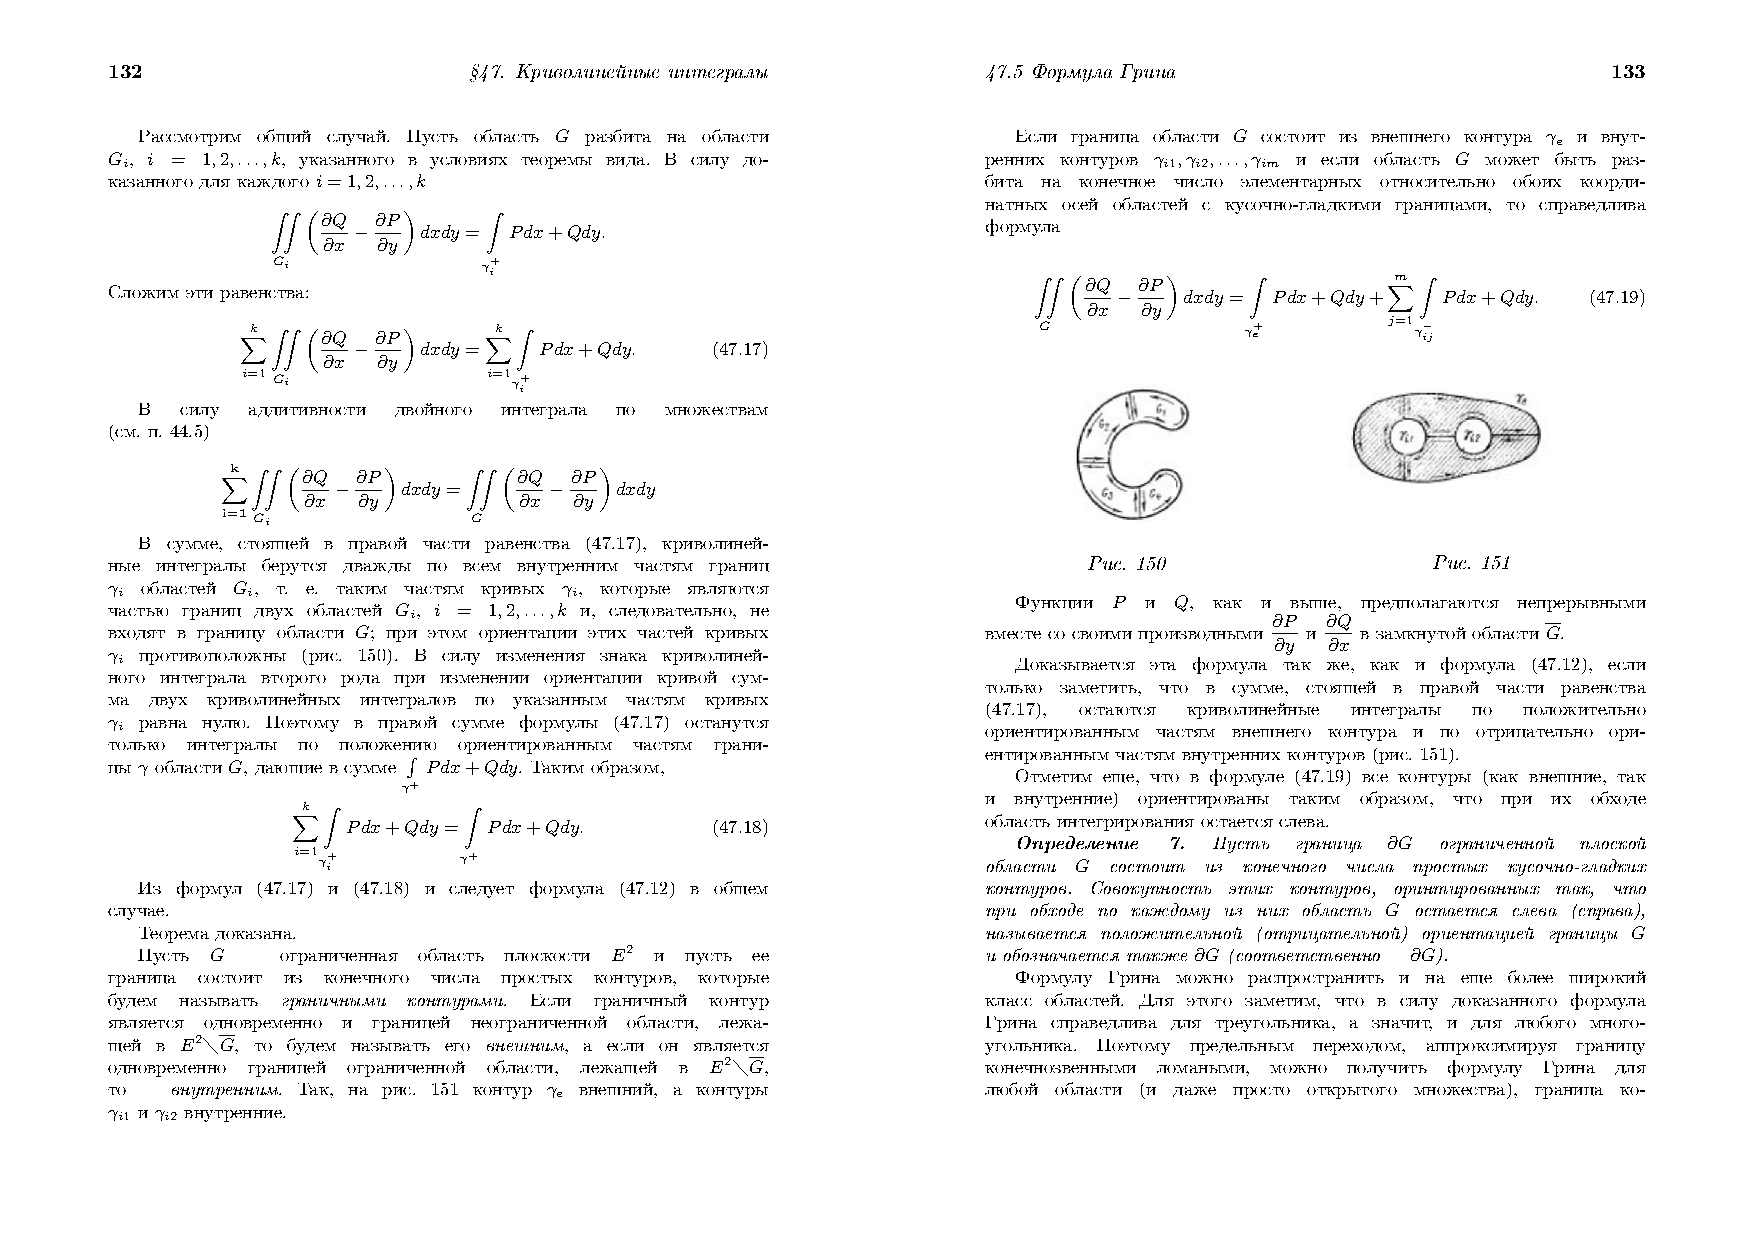
\includegraphics[width=\linewidth]{1.png}\\


\subsection*{Результат работы программы}
\begin{lstlisting}
karma@mydruzhok:~/mai_study/Crypto/lab5$ python main.py
Case #1: two meaningful texts in natural language.
Text length: 1310015
Match: 0.060799303824765366
Case #2: meaningful text and text from random letters.
Text length: 1572332
Match: 0.033484340457358874
Case #3: meaningful text and text from random words.
Text length: 1572332
Match: 0.05745294250832521
Case #4: two texts from random letters.
Text length: 1000000
Match: 0.03232720000000001
Case #5: two texts from random words.
Text length: 1000000
Match: 0.0603874
\end{lstlisting}

\subsection*{Выводы}
Как видно из результатов, наилучшие совпадения получаются путём сравнения двух осмысленных текстов и двух текстов из случайных слов. Худшие совпадения у осмысленного текста с текстом из случайных букв и у двух текстов из случайных букв. Думаю, полученные результаты можно было бы объяснить какими-то лингвистическими законами построения языка, но у меня нет достаточных знаний в этой области. Например, для букв английского языка характерна некоторая частотность, которая будет соблюдаться в осмысленных текстах, и которая не соблюдается в генерируемых из букв текстах. Эмпирически кажется, что размер слогов в осмысленных словах совпадает чаще, чем в случайных, и 5 букв, передающих гласные звуки в английском языке, будут совпадать чаще. Высокое совпадение тестов из случайных слов можно объяснить тем, что эти тексты были составлены по одному словарю. В текстах из случайных букв нет никаких ограничений на использование букв в верхнем регистре не на первой позиции в слове, что сильно снижает количество совпадений с осмысленным тестом.
\par Также кажется, что если в качестве осмысленных текстов взять разные произведения одного и того же автора, то совпадений будет больше, потому что у каждого автора можно выделить характерный для него словарь. Например, русские прозаики используют в своих произведениях примерно 6 тысяч уникальных слов (http://w-o-s.ru/article/9037). 
\par Что касается достаточной длины текста для корректного сравнения, начиная с какой-то достаточно большой длины, по закону больших чисел, среднее значение совпадений станет равным мат. ожиданию совпадений. Мат. ожидание количества совпадений для осмысленного текста определить сложно, потому что непонятно, какое там распределение. Поэтому рассмотрим два текста из случайных букв. 
\par Если речь идёт о сгенерированном тексте, то random.choice использует равномерное распределение. Вероятность выбора любого знака $\frac{1}{53}$ (26 букв в обоих регистрах и пробел). Пусть случайная величина $I_{k}$ -- индикатор совпадения знаков в $k$-ой позиции, т.е. $I_{k} = 1$, если знаки на $k$-ой позиции совпали и $I_{k} = 0$, если не совпали. Вероятность совпадения
двух знаков $\frac{1}{53} \cdot \frac{1}{53} = \frac{1}{2809}$, несовпадения -- $\frac{2808}{2809}$. Получаем распределение:
\begin{equation*}
I_{k} \sim
\begin{pmatrix}
0 & 1\\
\frac{2808}{2809} & \frac{1}{2809}
\end{pmatrix}
\end{equation*}
Математическое ожидание равно $E(I_{k}) = \frac{1}{2809}$. Случайная величина $X$ -- число совпадений знаков -- равна сумме индикаторов совпадения по всем позициям:
$$ X = I_{1} + I_{2} + \ldots + I_{N},$$
где $N$ -- длина текста (в нашем тесте $1000000$). Переходя к ожиданию:
$$ E(X) = N \cdot E(I_{1}) = 1000000 \cdot \frac{1}{2809} \approx 355 $$
Как видно из нашего теста, получившееся количество совпадений -- $32327$, что плохо соотносится с $355$. Думаю, это связано с тем, что пробелы в сгенерированых текстах встречаются чаще, чем другие знаки, и длина текста слишком маленькая. После того, как я убрала пробелы, количество совпадений стало равным $19216$. Но это всё равно много, по-хорошему надо увеличивать длину текста.



\subsection*{Листинг программного кода}
\begin{lstlisting}[language=Python]
import random
import string
import getopt
import os
import sys

import urllib.request


CNT_RANDOM_TEXTS = 10
LEN_RANDOM_TEXT = 10 ** 6
CASES = 5


USAGE = """
Syntax: main.py [--cases=#]

  Flags:
    cases=#
        Numbers of cases to use. By default all cases are used.

        1 -- two meaningful texts in natural language
        2 -- meaningful text and text from random letters
        3 -- meaningful text and text from random words
        4 -- two texts from random letters
        5 -- two texts from random words

    Example:
        --cases=1,3

"""


def count_common_letters(text1, text2):
    cnt = 0
    for char1, char2 in zip(text1, text2):
        if char1 == char2:
            cnt += 1
    return cnt


def match_perc(text1, text2):
    return count_common_letters(text1, text2) / len(text1)


def gen_random_letters(n):
    text = ''
    while len(text) < n:
        len_word = random.randint(3, 10)
        word = ''.join(random.choice(string.ascii_letters) \ 
                for _ in range(len_word))
        text += ' ' + word
    rem = len(text) - n
    if rem != 0:
        text = text[:-rem]
    return text


def gen_random_words(n):
    url = 'http://svnweb.freebsd.org/csrg/share/dict/
                words?view=co&content-type=text/plain'
    response = urllib.request.urlopen(url)
    words = response.read().decode()
    words = words.splitlines()
    text = ''
    while len(text) < n:
        text += ' ' + random.choice(words)
    rem = len(text) - n
    if rem != 0:
        text = text[:-rem]
    return text


def case1():
    print("Case #1: two meaningful texts in natural language.")
    url = 'http://www.gutenberg.org/files/4300/4300-0.txt'
    url2 = 'http://www.gutenberg.org/files/4280/4280-0.txt'
    response = urllib.request.urlopen(url)
    text1 = response.read().decode()
    response = urllib.request.urlopen(url2)
    text2 = response.read().decode()
    min_len = min(len(text1), len(text2))
    text1 = text1[:min_len]
    text2 = text2[:min_len]
    print("Text length: {0}".format(min_len))
    print("Match: {0}".format(match_perc(text1, text2)))


def case2():
    print("Case #2: meaningful text and text from random letters.")
    url = 'http://www.gutenberg.org/files/4300/4300-0.txt'
    response = urllib.request.urlopen(url)
    text1 = response.read().decode()
    s = 0
    for _ in range(CNT_RANDOM_TEXTS):
        text2 = gen_random_letters(len(text1))
        s += match_perc(text1, text2)
    s /= CNT_RANDOM_TEXTS
    print("Text length: {0}".format(len(text1)))
    print("Match: {0}".format(s))


def case3():
    print("Case #3: meaningful text and text from random words.")
    url = 'http://www.gutenberg.org/files/4300/4300-0.txt'
    response = urllib.request.urlopen(url)
    text1 = response.read().decode()
    s = 0
    for _ in range(CNT_RANDOM_TEXTS):
        text2 = gen_random_words(len(text1))
        s += match_perc(text1, text2)
    s /= CNT_RANDOM_TEXTS
    print("Text length: {0}".format(len(text1)))
    print("Match: {0}".format(s))


def case4():
    print("Case #4: two texts from random letters.")
    s = 0
    for _ in range(CNT_RANDOM_TEXTS):
        text1 = gen_random_letters(LEN_RANDOM_TEXT)
        text2 = gen_random_letters(LEN_RANDOM_TEXT)
        s += match_perc(text1, text2)
    s /= CNT_RANDOM_TEXTS
    print("Text length: {0}".format(LEN_RANDOM_TEXT))
    print("Match: {0}".format(s))


def case5():
    print("Case #5: two texts from random words.")
    s = 0
    for _ in range(CNT_RANDOM_TEXTS):
        text1 = gen_random_words(LEN_RANDOM_TEXT)
        text2 = gen_random_words(LEN_RANDOM_TEXT)
        s += match_perc(text1, text2)
    s /= CNT_RANDOM_TEXTS
    print("Text length: {0}".format(LEN_RANDOM_TEXT))
    print("Match: {0}".format(s))


def print_usage(message):
    print(USAGE)
    if message:
        sys.exit('\nFATAL ERROR: ' + message)
    else:
        sys.exit(1)


def parse_args(args):
    try:
        opts, args = getopt.getopt(args, '', ['help', 'cases='])
    except getopt.GetoptError:
        print_usage('Invalid arguments.')

    cases = [i for i in range(1, CASES + 1)]

    for (opt, val) in opts:
        if opt == '--help':
            print_usage(None)
        elif opt == '--cases':
            try:
                cases = set(map(int, val.split(',')))
            except ValueError:
                print_usage('Cases must be comma separated list.')

            for i in cases:
                if i not in range(1, CASES + 1):
                    print_usage('Incorrect cases')

    return cases


if __name__ == '__main__':
    cases = parse_args(sys.argv[1:])

    for i in cases:
        if i == 1:
            case1()
        elif i == 2:
            case2()
        elif i == 3:
            case3()
        elif i == 4:
            case4()
        elif i == 5:
            case5()


\end{lstlisting}

\end{document}
